In the following paragraph are presented the most relevant and significant algorithm used in Travlendar+ application.
More specifically are described the following algorithm:
\begin{itemize}
	\item Compute travel;
	\item View daily schedule;
	\item Check appointments overlapping;
	\item Check appointments unreachability;
	\item Check travel alternatives;
	\item Check movement alternatives;
\end{itemize}

The application is written in Java, but the algorithms are shown in pseudocode.

\subsection{Object class}

Before to explain the algorithms details, it is needed to introduce the class Appointment, Travel and Movement that are the most important entities for the whole application.

\subsubsection{Appointment class}

The class Appointment has as attributes:
\begin{itemize}
	\item The appointment name;
	\item The date;
	\item The start time;
	\item The place of arrival;
	\item The expected time of arrival;
	\item The appointment duration;
	\item The associated travel to reach the appointment;
\end{itemize}

Here the appointment class written in Java:
\begin{lstlisting}[language=Java]
	public class Appointment {
	
		String name;
		Date date;
		Time time;
		Place place;
		Time timeOfArrival;
		Time duration;
		Travel travel;
	}
		
\end{lstlisting}

\subsubsection{Travel class}

The travel class has the following attributes:
\begin{itemize}
	\item The related appointment;
	\item The departure point;
	\item The destination point;
	\item The desired time to leave;
	\item The movements list in which the travel is split;
\end{itemize}

Here the travel class written in Java:
\begin{lstlisting}[language=Java]
	public class Travel {
	
		Appointment appointment;
		Place placeOfDeparture;
		Place placeOfArrival;
		Time timeOfDeparture;
		ArrayList<Movement> movements;
	}
\end{lstlisting}

\subsubsection{Movement class}

The movement class has the following attributes:
\begin{itemize}
	\item The departure point;
	\item The destination point;
	\item The estimated time;
	\item The time of departure;
\end{itemize}

Here the movement class written in Java:
\begin{lstlisting}[language=Java]
	public class Movement {
		
		Place placeOfDeparture;
		Place placeOfArrival;
		Time estimatedTime;
		Time timeOfDeparture;
	}
\end{lstlisting}

\subsection{Algorithms}

\subsubsection{Create flexible appointment}

\subsubsection{Compute travel}

The function computeTravel is used to create a new travel for a specific appointment.
The followed procedure is composed by four steps:
\begin{enumerate}
	\item Read the different information from the appointment passed as parameters.
	\item Call the function queryMaps. this uses Google Maps API to compute the travel, the response is JSON object and the function parse this and extracts all information related to the computed travel.
	\item For each steps, which put together with the other steps produces the travel, is created a new Movement and it is added to MovementList presents in Travel class.
	\item Call the function computeWeatherCondition, that with specific API can compute the weather condition, and if the travel includes some walking or bicycling movement and it is expected 'rain', the system shows to the user a message.
\end{enumerate}

\begin{algorithmic}
	\Function{computeTravel}{appoinment, placeOfDeparture, timeOfDeparture, preferences}
		
		\State \Call{read}{appointment.place}
		\State \Call{read}{preferences.travelPreferences}
		
		\State travel = \Call{queryMaps}{placeOfDeparture,place,travelPreferences} 
		
		\ForAll{movement detected in travel}
			\State createdMovement = \Call {createMovement}{movement}
			\State \Call {addToMovementList}{createdMovement}
		\EndFor
		
		\State \Call{read}{appointment.date}
		\State \Call{read}{appointment.time}
		
		weather = \Call{computeWeatherCondition}{placeOfDeparture, place, date, time}
		\If {wheater is 'rain' and ( (travelPreferences is 'green') or (exists one movement : movementType is 'walk' or 'bike') )}
			\State \Call {notifyUser}{"Rain expected, not reccomended use of bike or walks"}
		\EndIf
	\EndFunction
\end{algorithmic}


\subsubsection{View daily schedule}

When the user clicks on view daily schedule button, the system computes the daily schedule through this function and show to the user all appointments expected for the selected day and all travel to reach them.
This method has only one parameter, the day desired to compute the schedule.\\
The function is composed by four steps:
\begin{enumerate}
	\item Extract first appointment expected in the selected day (appointment-i) and check its unreachability.
	\item Extract the second appointment (appointment-i+1) and check its unreachability.
	\item If both appointments are reachable then it is necessary to check the overlapping between them.
	\item If all controls are successfully passed then it is possible to compute the travel for the appointment-i.
	\item Go on with the next appointment and repeats the loop until all appointments are examinated.
\end{enumerate}

\begin{algorithmic}
	\Function{viewDailySchedule}{day}
		
		\ForAll{appointment in day}
			\If{\Call{checkUnreachability}{appointment-i} is unreachable} 
				\State \Call{manageUnreachability}{appointment-i}
			\EndIf
		\EndFor
		
		\If{\Call{checkUnreachability}{appointment-i+1} is unreachable} 
			\State \Call{manageUnreachability}{appointment-i+1}
		\ElsIf {\Call{checkOverlap}{appointment-i, appointment-i+1} is overlap}
			\State \Call {manageOverlap}{appointment-i,appointment-i+1}
		\EndIf
		\Call {computeTravel}{appointment-i,appointment-i.travel.placeOfDeparture, appoinment-i.travel.departureTime,preferences}
		\Call {increment}{i}
	\EndFunction
\end{algorithmic}

\subsubsection{Check overlap}

When the system has to check the overlapping between two appointments invokes this function that has as parameter the two appointments.
The function controls which appointment starts before and then controls if the begin time of the second appointment overlaps with end time of the first appointment.

\begin{algorithmic}
	
	\Function {checkOverlap}{app1, app2}
		\If{app1.time is before of app2.time and (app2.time is before (app1.time + app1.duration))} 
			\State \Return overlap
		\ElsIf{app1.time is before (app2.time + app2.duration)} 
			\State \Return overlap
		\EndIf;
		\State \Return no overlap
	\EndFunction
\end{algorithmic}

\subsubsection{Check unreachability}

This function checks the unreachability of one appointment passed as parameter.
To check the unreachability it is necessary to control if the arrival time of one appointment is compatible with departure time added to estimated travel time.

\begin{algorithmic}
	
	\Function {checkUnreachability}{appointment}
		\If {appointment.timeOfArrival is before (appointment.travel.timeOfDeparture + travel duration)} 
			\State \Return unreachable;
		\Else 
			\State \Return reachable;
		\EndIf
	\EndFunction
\end{algorithmic}

\subsubsection{Check travel alternative}
The user can check all available travel alternatives and modify the actual one with another. This is possible switching the different alternatives.
\begin{figure}[!h]
	\centering
	\makebox[\textwidth][c]{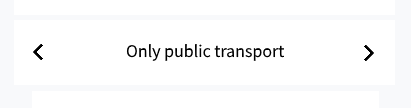
\includegraphics[width=0.5\textwidth]{Images/TravelAlternatives.png}}%
\end{figure}
\\The function checkTravelAlternative reads the selected alternative and computes the travel with the inserted TravelType.
\\View more detailed these steps:
\begin{enumerate}
	\item There is a control on a travel type selected from the user and there are two possible cases:
		\begin{enumerate}
			\item 'only-own-car' or 'only-public-transport' or 'green:
				when one these travel type is selected, it is created a new travel alternative based on related travel mode (driving for only-own-car, transit for only-public-transport and bicycling for green).
			\item 'faster' or 'cheaper':  in this case, it is created a set that contains all possible travel computable.
		\end{enumerate}
	\item Then it is selected the travel alternative:
		\begin{enumerate}
			\item In case of cheaper or faster travel, it is necessary to find among all computed travels the cheaper or the faster.
			\item In other cases, return the only one alternative computed.
		\end{enumerate}
\end{enumerate}

\begin{algorithmic}

	\Function {checkTravelAlternative}{travel, travelType}
		
		\If {travelType is 'only-own-car'}
			\State 	compute driving travel alternative
		\ElsIf {travelType is 'only-public-transport'}
			\State 	compute transit travel alternative
		\ElsIf {travelType is 'green'}
			\State 	compute bicycling travel alternative
		\ElsIf {travelType is 'faster' or travelType is 'cheaper'}
			\State 	compute a set of differents travel alternatives
		\EndIf
		\If {travel alternative exists}
			\If {travelType is 'faster'} 
				\State find faster travel in the computed set and return it
			\EndIf
			\If travelType is 'cheaper'
				\State find cheaper travel in the computed set and return it
			\EndIf
			\State \Return the travel alternative found
		\EndIf
	\EndFunction
\end{algorithmic}

\subsubsection{Check movement alternative}
When the user views a movement details and clicks on a "means icon" from the bar, the system calls this function that read the movement type selected and computed the relative movement.	
\\ If the user selects 'car-sharing' or 'bike-sharing' it is added a new movement to reach the car or bike.

\begin{algorithmic}
	\Function {checkMovementAlternative}{movement, movementType}
		\If {movementType is 'car'}
			\State compute driving movement
		\ElsIf {movementType is 'walk'}
			\State compute walking movement
		\ElsIf {movementType is 'public-transport'}
			\State compute transit movement
		\ElsIf {movementType is 'bike'}
			\State compute bicycling movement
		\ElsIf {movementType is 'car-sharing'}
			\State compute walking movement to reach the car
			\State add a further driving movement
		\ElsIf {movementType is 'bike-sharing'}
			\State compute walking movement to reach the bike
			\State add a further bicycling movement
		\EndIf
	
		\If{computed movement exists}
			\State \Return movement alternative
		\EndIf
	\EndFunction

\end{algorithmic}

